\chapter{الإلكترونات في الأجسام الصلبة}\label{ch:b3:electrons-in-solids}

% Provenance (not for print): second half of the "physique du solide"
% module (Drude, Sommerfeld, bands, semiconductors) common to the
% surveyed third-year curricula.

النحاس ينقل الكهرباء أفضل من الكوارتز بمليون مليار مليار
مرة --- وهو أوسع مجال لأيّ خاصة فيزيائية، تأمر به
مواد تبدو كتلًا رمادية في الحالتين. وسقالة
الفصل الماضي لا تشرح شيئًا من ذلك؛ أما \emph{الإلكترونات} المصبوبة
فيها فتشرحه كله. ويجري هذا الفصل محاولات القرن الثلاث في
المسألة، وكلٌّ ترث حطام سابقتها: كرة درودي
الكلاسيكية (1900)، التي تصيب قانون أوم وتخطئ السعة الحرارية
خطأً فاضحًا؛ وغاز فيرمي عند زومرفلد، وهو
\cref{ch:b3:quantum-statistics} تصرف شيكها؛ وبصيرة بلوخ
بأن موجة الإلكترون في \omterm{def:b3:crystalline-solids:lattice}{شبكة} دورية تنعكس انعكاس براغ
مثل أيّ موجة أخرى --- ففتحت \emph{فجوات عصابات} تفرز الأجسام الصلبة كلها
إلى فلزات وعوازل وأولاد وسط ضيّقي الفجوة،
أي أنصاف النواقل، التي بُني عليها عصر الإلكترونيات كله. وينتهي
الفصل داخل لوح شمسي.

\section{فلز درودي ذو الكرة}

\begin{proposition}[ناقلية درودي]\label{prop:b3:electrons-in-solids:drude}
\index{نموذج درودي}\index{الناقلية!المجهرية}\index{سرعة الانجراف}
عامل إلكترونات التكافؤ في \omterm{def:b3:electrons-in-solids:classes}{فلز} غازًا كلاسيكيًّا كثافته $n$،
ترتدّ عن عوائق كل $\tau$ ثانية. والمجال $\vect E$
يسرّع كلًّا منها بين التصادمات؛ ومتوسط \emph{\omterm{prop:b3:electrons-in-solids:drude}{سرعة
الانجراف}} هو $\vect v_{\text{d}} = -e\tau\vect E/m_{\text{e}}$،
وهو ضئيل إلى جانب الحركة الحرارية. وعندئذٍ تطيع كثافة التيار $\vect j =
-ne\vect v_{\text{d}}$ قانونَ أوم موضعيًّا،
$\vect j = \sigma\vect E$، مع
\[
\sigma = \frac{ne^2\tau}{m_{\text{e}}} .
\]
وتقتضي $\sigma$ المقيسة للنحاس $\tau \approx \qty{2.5e-14}{s}$
--- وتتبع مجدَتا النموذج: فهو يشرح لماذا تسخن المقاومات
(إذ يُحرَّر شغل المجال حراريًّا في كل تصادمة)، و
يتنبأ بقانون فيدمان--فرانتس، أي أن $\kappa/\sigma T$ ثابت
واحد لكل الفلزات --- فالإلكترونات تحمل الشحنة و
الحرارة معًا (\cref{exo:b3:electrons-in-solids:5}).
\end{proposition}

\begin{proof}
بين التصادمات $\dot{\vect v} = -e\vect E/m_{\text{e}}$؛
وبالبدء من جديد عند كل تصادمة، تكون السرعة الوسطى المكتسبة في
زمن وسطي $\tau$ هي $-e\tau\vect E/m_{\text{e}}$. ومنه $\vect j =
-ne\vect v_{\text{d}} = (ne^2\tau/m_{\text{e}})\vect E$.
\end{proof}

\begin{omfigure}
\begin{tikzpicture}[scale=1.0]
  % ion grid
  \foreach \x in {0,1.3,...,7.9}
    \foreach \y in {0,1.1,2.2}
      \draw[omDef!50, fill=omDef!12] (\x,\y) circle (5.5pt);
  % zigzag electron path with slight downfield drift
  \draw[omThm, thick, ->]
    (0.25,1.62) -- (1.0,0.55) -- (1.9,1.7) -- (2.6,0.6) -- (3.6,1.55)
    -- (4.3,0.45) -- (5.25,1.6) -- (5.95,0.5) -- (6.9,1.5) -- (7.65,0.7);
  % field and drift arrows
  \draw[->, thick] (2.6,3.0) -- (1.2,3.0)
    node[midway, above, font=\scriptsize] {$\vect E$};
  \draw[->, thick, omThm, dashed] (5.0,3.0) -- (6.8,3.0)
    node[midway, above, font=\scriptsize]
    {انجراف $\vect v_{\text{d}}$};
\end{tikzpicture}

{\small صورة درودي: إلكترون يرتدّ عند
$\sim\qty{e6}{m/s}$، بينما يركّب المجال فوقها انجرافًا مقداره
أجزاء من الميليمتر في الثانية
(\cref{exo:b3:electrons-in-solids:2}). فيسقط قانون أوم؛ و
إخفاقات النموذج علّمت أكثر بعد.}
\end{omfigure}

\begin{remark}[إنقاذ زومرفلد]\label{rem:b3:electrons-in-solids:sommerfeld}
\index{نموذج زومرفلد}\index{طاقة فيرمي!في الفلزات}
ينبغي لغاز درودي أن يضيف $\tfrac32k_{\text{B}}$ لكل إلكترون إلى
السعة الحرارية \omterm{def:b3:electrons-in-solids:classes}{للفلز}؛ والتجربة تجد أقلّ بمئة مرة.
وقد برّأت \cref{ch:b3:quantum-statistics} الإلكترونات سلفًا:
فهي \emph{غاز فيرمي منحلّ}، $T_{\text{F}} \sim
\qty{8e4}{K}$، ولا تستطيع الاستجابة --- للحرارة و
للانتثار --- إلا القشرة الحرارية في حدود $k_{\text{B}}T$ من سطح فيرمي.
وإعادة زومرفلد لتشغيل درودي بإحصاء فيرمي--ديراك
تحفظ صيغة الناقلية (مع $\tau$ صائرًا الآن
عمر إلكترونات سطح فيرمي، التي تكون \qty{e6}{m/s} لها هي
$v_{\text{F}}$ لا السرعة الحرارية)، وتصلح السعة الحرارية إلى شريحة
$T/T_{\text{F}}$ المقيسة، بل تصلح ثابت
فيدمان--فرانتس العددي. ويبقى لغز واحد ينجو من كل
نموذج للإلكترون الحرّ: لماذا لا ينقل الكوارتز البتة.
\end{remark}

\section{بلوخ: الشبكة تتكلم}

\begin{theorem}[حالات بلوخ وفجوات العصابات]\label{thm:b3:electrons-in-solids:bloch}
\index{مبرهنة بلوخ}\index{فجوة العصابة}\index{بنية العصابات}
في كمون دوري تامّ، تكون الحالات المستقرة
\emph{أمواج بلوخ} $\psi_k(x) = u_k(x)\eu^{\iu kx}$ ---
أي أمواج مستوية مكسوّة بدورية \omterm{def:b3:crystalline-solids:lattice}{الشبكة} نفسها $u_k$ ---
وهي تنتشر \emph{بلا انتثار}: فللبلورة التامّة
مقاومة معدومة، والمقاومة الحقيقية تأتي من العيوب
(الاهتزازات والشوائب). لكن ليست كل الطاقات تنجو. فعند
$k = \pi/a$ يكون طول موجة الإلكترون $2a$: أي شرط براغ
على \omterm{def:b3:crystalline-solids:lattice}{الشبكة} نفسها (وقد قامت \cref{thm:b3:crystalline-solids:dispersion}
بالاكتشاف نفسه للصوت). وتكوّن الموجتان المنعكسة والواردة
نمطين موقوفين --- بشحنة مكدَّسة على الأيونات
(بطاقة أدنى) أو بينها (بطاقة أعلى) --- فيتمزق قطع مكافئ
الإلكترون الحرّ $E = \hbar^2k^2/2m_{\text{e}}$: أي تفصل فترة من
الطاقات المحرَّمة، هي \emph{\omterm{thm:b3:electrons-in-solids:bloch}{فجوة العصابة}} $E_{\text{g}}$،
\emph{عصابةً} مملوءة من الحالات المسموحة عن التالية. و
هوية \omterm{def:b3:crystalline-solids:lattice}{البلورة} الإلكترونية هي سلّم عصاباتها وفجواتها.
\end{theorem}
\admitted

\begin{omfigure}
\begin{tikzpicture}
  \begin{axis}[omaxis, axis x line=bottom, axis y line=left,
    width=9.6cm, height=6.2cm, xmin=0, xmax=5.4, ymin=0, ymax=2.6,
    xlabel={$k$}, ylabel={$E$},
    xlabel style={at={(axis description cs:0.5,-0.1)}, anchor=north},
    xtick={3.1416}, xticklabels={$\pi/a$}, ytick=\empty, clip=true]
    % free-electron parabola (dashed)
    \addplot[gray, dashed, domain=0:5.1, samples=120] {x*x/10};
    % lower band: bends flat at zone edge
    \addplot[omDef, very thick, domain=0:3.1416, samples=120]
      {x*x/10 - 0.18*(x/3.1416)^6};
    % upper band
    \addplot[omDef, very thick, domain=3.1416:5.1, samples=120]
      {x*x/10 + 0.18*((5.1-x)/1.9584)^2};
    \draw[gray, dashed] (axis cs:3.1416,0) -- (axis cs:3.1416,2.55);
    % gap markers
    \draw[omThm, thick, <->] (axis cs:3.2,0.81) -- (axis cs:3.2,1.16);
    \node[omThm, font=\scriptsize, anchor=west] at (axis cs:3.34,0.98)
      {فجوة $E_{\text{g}}$};
    \node[gray, font=\scriptsize, anchor=north west, align=left]
      at (axis cs:0.35,2.45) {المتقطع: إلكترون حرّ};
    \node[omDef, font=\scriptsize, anchor=east] at (axis cs:2.75,0.35)
      {العصابة 1};
    \node[omDef, font=\scriptsize, anchor=west] at (axis cs:3.6,2.35)
      {العصابة 2};
  \end{axis}
\end{tikzpicture}

{\small الإلكترون شبه الحرّ. فبعيدًا عن حافة المنطقة
لا يكاد الإلكترون يلحظ \omterm{def:b3:crystalline-solids:lattice}{الشبكة}؛ وعند $k = \pi/a$ يشقّ انعكاس براغ
الخاص به قطعَ المكافئ، فيحرّم الطاقات في
الفجوة. وقد فعلت أمواج الصوت هذا بالضبط في الفصل الماضي --- \omterm{def:b3:crystalline-solids:lattice}{الشبكة}
نفسها، والتداخل نفسه، ونزيل جديد.}
\end{omfigure}

\begin{definition}[الفلزات والعوازل وأنصاف النواقل]\label{def:b3:electrons-in-solids:classes}
\index{فلز}\index{عازل}\index{نصف ناقل}
املأ العصابات بإلكترونات \omterm{def:b3:crystalline-solids:lattice}{البلورة}، اثنين لكل حالة
(\cref{ch:b3:identical-particles})، من الأبرد أولًا. فإذا كانت
العصابة المشغولة العليا مملوءة \emph{جزئيًّا}، استطاعت طاقة لامتناهية الصغر
أن تزيح الإلكترونات إلى حركة صافية: فهو \emph{فلز} (فالصوديوم: بإلكترون
تكافؤ واحد، أي نصف عصابة؛ والفلزات ثنائية التكافؤ تنقل عبر
عصابات متراكبة). وإذا كانت مملوءة \emph{تمامًا}، وفوقها فجوة واسعة،
فلا دفعة صغيرة تستطيع إعادة ترتيب شيء: فهو \emph{عازل}
(الألماس، $E_{\text{g}} = \qty{5.5}{eV}$). وإذا كانت الفجوة صغيرة ---
$\qty{1.12}{eV}$ في السيليكون --- رفع الاهتياج الحراري بضعة
إلكترونات عبرها، فيترك كلٌّ منها \emph{ثقبًا} متحركًا تحته: فهو
\emph{نصف ناقل}، يتضاعف عدد حاملاته
$\propto\eu^{-E_{\text{g}}/2k_{\text{B}}T}$ كل بضع
درجات. ومن هنا الانقسام الكبير: فالفلزات تنقل أسوأ عند التسخين
(إذ تكثر الاهتزازات التي تنتثر عنها)، وأنصاف النواقل أفضل
(إذ تكثر الحاملات كثرةً أُسّية) --- أي انقلاب إشارة واحد يعيّن
صنف المادة في قياس واحد.
\end{definition}

\begin{omfigure}
\begin{tikzpicture}[scale=1.0]
  % metal: half-filled band
  \begin{scope}
    \fill[omDef!25] (0,0) rectangle (1.8,0.8);
    \draw[thick] (0,0) rectangle (1.8,1.6);
    \node[font=\scriptsize, anchor=north] at (0.9,-0.15) {فلز};
    \node[font=\tiny, anchor=south] at (0.9,1.65) {مملوءة جزئيًّا};
  \end{scope}
  % insulator
  \begin{scope}[xshift=3.6cm]
    \fill[omDef!25] (0,0) rectangle (1.8,0.9);
    \draw[thick] (0,0) rectangle (1.8,0.9);
    \draw[thick] (0,2.1) rectangle (1.8,2.9);
    \draw[omThm, thick, <->] (2.05,0.9) -- (2.05,2.1);
    \node[omThm, font=\tiny, anchor=west] at (2.12,1.5)
      {$E_{\text{g}} \sim \qty{5}{eV}$};
    \node[font=\scriptsize, anchor=north] at (0.9,-0.15) {عازل};
    \node[font=\tiny, anchor=south] at (0.9,2.95) {فارغة};
  \end{scope}
  % semiconductor
  \begin{scope}[xshift=8.4cm]
    \fill[omDef!25] (0,0) rectangle (1.8,0.9);
    \draw[thick] (0,0) rectangle (1.8,0.9);
    \draw[thick] (0,1.5) rectangle (1.8,2.3);
    \draw[omThm, thick, <->] (2.05,0.9) -- (2.05,1.5);
    \node[omThm, font=\tiny, anchor=west] at (2.12,1.2)
      {$\sim\qty{1}{eV}$};
    % thermally excited carriers
    \fill[omThm] (0.5,1.62) circle (1.6pt);
    \fill[omThm] (1.25,1.62) circle (1.6pt);
    \draw[omThm] (0.5,0.78) circle (1.6pt);
    \draw[omThm] (1.25,0.78) circle (1.6pt);
    \node[font=\scriptsize, anchor=north] at (0.9,-0.15) {نصف ناقل};
    \node[font=\tiny, anchor=south] at (0.9,2.35)
      {بضعة إلكترونات $+$ ثقوب};
  \end{scope}
\end{tikzpicture}

{\small ملء العصابات يقرر كل شيء. فالعصابة المملوءة جزئيًّا
تنقل؛ والعصابة الممتلئة تحت فجوة واسعة لا تستطيع؛ والفجوة الضيقة تتيح
لدرجة الحرارة (أو الضوء أو \omterm{def:b3:electrons-in-solids:doping}{التطعيم}) أن تفاوض --- فكامل فائدة
\omterm{def:b3:electrons-in-solids:classes}{نصف الناقل} أن ناقليته \emph{قابلة للضبط}.}
\end{omfigure}

\section{هندسة الفجوة: التطعيم والوصلة}

\begin{definition}[التطعيم]\label{def:b3:electrons-in-solids:doping}
\index{التطعيم}\index{مانح}\index{قابل}\index{ثقب}
استبدل بذرة سيليكون واحدة من كل مليون ذرةَ فوسفور (بخمسة إلكترونات
تكافؤ): فتُشبَع أربع روابط ويكون الإلكترون الخامس،
المرتبط بمقدار \qty{45}{meV} لا غير
(\cref{exo:b3:electrons-in-solids:10})، حرًّا عند حرارة
الغرفة. وهذه \emph{المانحات} تصنع \omterm{def:b3:electrons-in-solids:classes}{نصف ناقل} \emph{من النوع N}،
تنقل فيه الإلكترونات؛ أما البورون (بثلاثة إلكترونات)
فهو \emph{قابل}، ينتزع إلكترون رابطة ويحرّر
\emph{ثقبًا} متحركًا --- أي إلكترونًا غائبًا يتحرك ويستجيب
للمجالات ويحمل شحنة موجبة حملًا حقيقيًّا كما تحمل فقاعة
الطفوَ: فهو \emph{من النوع P}. والتطعيم يؤرجح كثافة الحاملات
--- ومن ثمّ الناقلية --- عبر ست مراتب قدر
كما نشاء: أي المقبض الذي يحوّل الرمل إلى دارات.
\end{definition}

\begin{proposition}[وصلة PN]\label{prop:b3:electrons-in-solids:junction}
\index{وصلة PN}\index{ثنائي}\index{منطقة الاستنزاف}
صِل النوع P بالنوع N. فتنسكب الإلكترونات نحو الثقوب و
تفنيها قرب السطح الفاصل، فتكشف \emph{منطقة استنزاف}
من المطعّمات المؤيَّنة الثابتة تبني طبقتها المزدوجة مجالًا
داخليًّا --- أي توازنًا عند الجهد الداخلي
$V_{\text{bi}} = (k_{\text{B}}T/e)
\ln(N_{\text{a}}N_{\text{d}}/n_{\text{i}}^2) \approx
\qty{0.7}{V}$ في السيليكون. وعندئذٍ تقوّم الوصلة: فالانحياز
الأمامي يخفض الحاجز فينمو التيار وفق
$\eu^{eV/k_{\text{B}}T}$؛ والانحياز العكسي يرفعه فلا يسيل إلا
تسرّب $I_0$:
\[
I = I_0\big(\eu^{eV/k_{\text{B}}T} - 1\big) .
\]
وهذا اللاتناظر هو \emph{الثنائي} --- ومُجرًى في صوره،
يكون الديود الباعث للضوء LED (إذ تصدر الأزواج المعاد التحامها فوتونات بطاقة الفجوة)، والخلية
الشمسية (إذ تخلق فوتونات بطاقة الفجوة أزواجًا يجرفها المجال
الداخلي: \cref{pb:b3:electrons-in-solids:1})، ومضاعفًا
في شطائر، يكون الترانزستور: أي المفتاح الذي تطبع منه
الرقاقة الحديثة مئات المليارات.
\end{proposition}
\admitted

\begin{omfigure}
\begin{tikzpicture}
  \begin{axis}[omaxis,
    width=9.4cm, height=5.8cm, xmin=-4.6, xmax=3.6, ymin=-5, ymax=16,
    axis lines=middle,
    xlabel={$eV/k_{\text{B}}T$}, ylabel={$I/I_0$},
    xlabel style={anchor=north east},
    xtick=\empty, ytick=\empty, clip=true]
    \addplot[omDef, very thick, domain=-4.5:2.83, samples=200]
      {exp(x) - 1};
    \addplot[gray, dashed, domain=-4.6:0] {-1};
    \node[gray, font=\scriptsize, anchor=north] at (axis cs:-2.7,-1.7)
      {عكسي: تسرّب $-I_0$};
    \node[omDef, font=\scriptsize, anchor=east, align=right]
      at (axis cs:2.5,11.5) {أمامي:\\$\eu^{eV/k_{\text{B}}T}$};
  \end{axis}
\end{tikzpicture}

{\small قانون الثنائي. الجهد الأمامي يُردّ أُسّيًّا؛ و
الجهد العكسي لا يشتري إلا التسرّب $I_0$. فوصلة واحدة
تقوّم؛ واثنتان تصنعان ترانزستورًا؛ ومتر مربع منها،
مشمَّسًا، يصنع محطة طاقة.}
\end{omfigure}

\begin{omfigure}
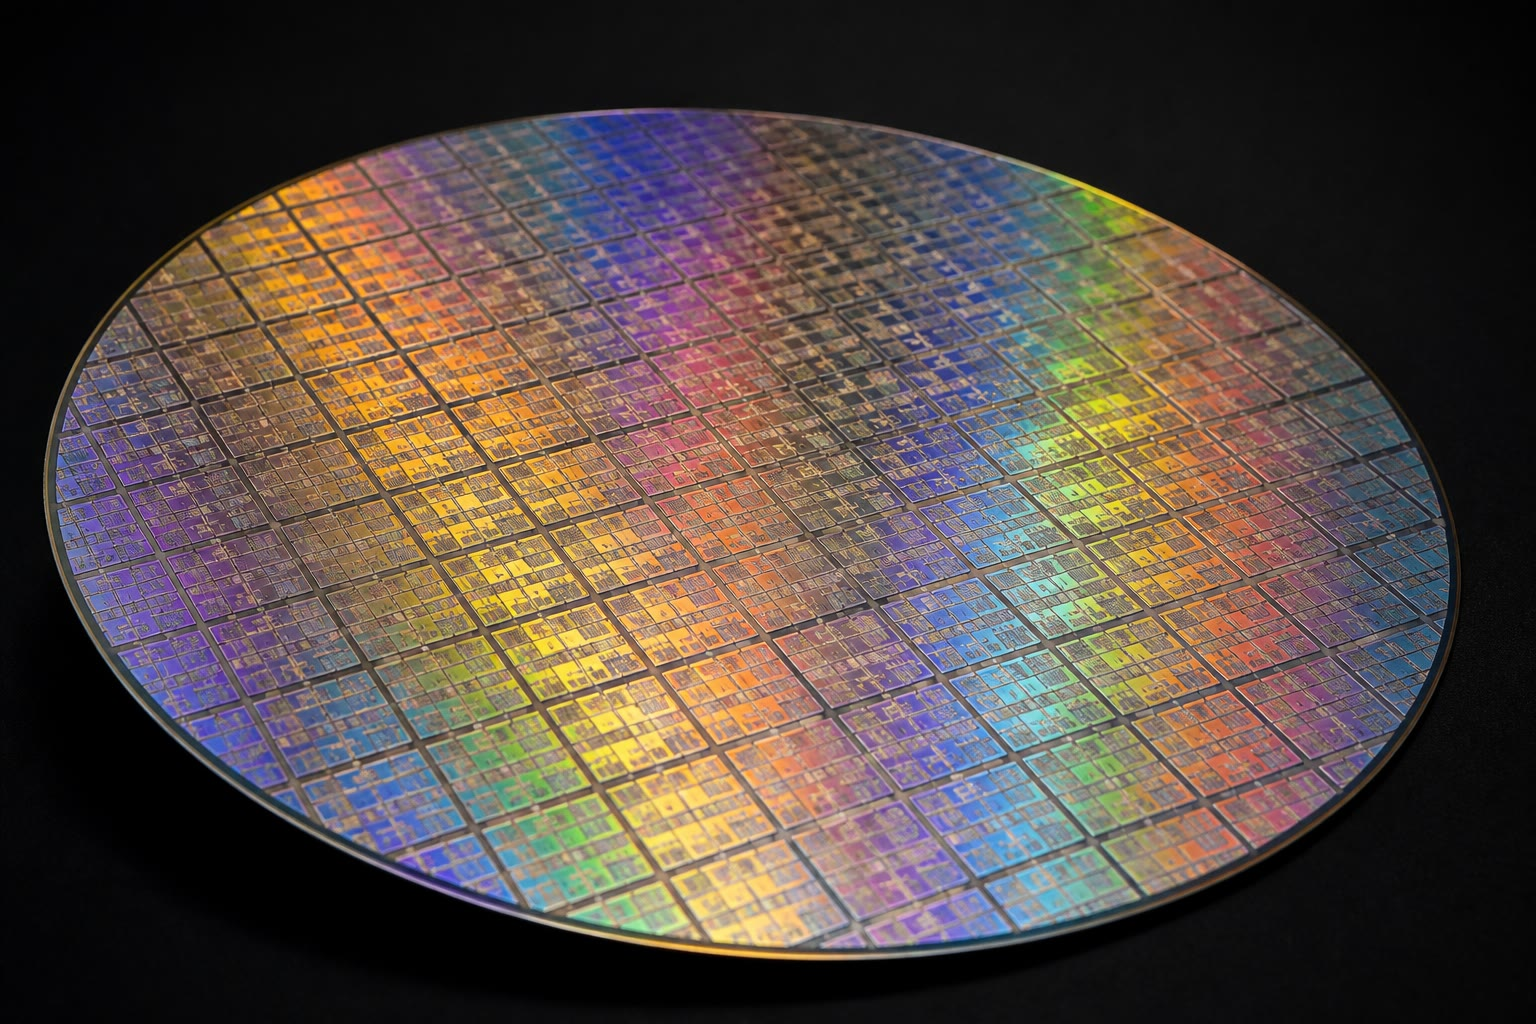
\includegraphics[width=0.58\linewidth]{images/book5/ai/b5-20-silicon-wafer.jpg}

{\small رقاقة سيليكون منتهية: مئات الرقائق، وفي كلٍّ مليارات الوصلات، مطبوعة في \omterm{def:b3:crystalline-solids:lattice}{بلورة} مطعَّمة واحدة --- أي نظرية العصابات وصفةً تصنيعية هي الأبلغ أثرًا في القرن العشرين.}
\end{omfigure}

\section{تمارين}

\begin{exercise}[$\star$]\label{exo:b3:electrons-in-solids:1}
نحاس درودي. $n = \qty{8.5e28}{m^{-3}}$، والمقاومية
$\rho = \qty{1.7e-8}{\ohm.m}$. احسب (أ) $\tau =
m_{\text{e}}/ne^2\rho$؛ (ب) متوسط المسير الحرّ باستعمال سرعة
فيرمي $v_{\text{F}} = \qty{1.6e6}{m/s}$؛ (ج) ذلك المسير بثوابت
\omterm{def:b3:crystalline-solids:lattice}{الشبكة} ($a = \qty{3.61}{\angstrom}$)؛ (د) اشرح لماذا
يلمّح طيران بهذا الطول أصلًا إلى أن الأيونات نفسها ليست هي
التي تنتثر.
\end{exercise}

\begin{exercise}[$\star$]\label{exo:b3:electrons-in-solids:2}
الحلزون في السلك. سلك نحاسي مساحته \qty{1}{mm^2} يحمل
\qty{10}{A}. (أ) احسب \omterm{prop:b3:electrons-in-solids:drude}{سرعة الانجراف}. (ب) وكم يستغرق
إلكترون ليعبر سلك مصباح طوله \qty{1}{m}؟ (ج) ولماذا يضيء
المصباح فورًا مع ذلك؟ (د) وقارن
$v_{\text{d}}$ بسرعة $v_{\text{F}}$ وعلّق على صورة
كرة درودي.
\end{exercise}

\begin{exercise}[$\star$]\label{exo:b3:electrons-in-solids:3}
الفرز بالعصابات. صنّف، بقاعدة ملء العصابات: (أ)
الصوديوم (بإلكترون تكافؤ واحد)؛ (ب) المغنيزيوم (باثنين --- ومع ذلك
\omterm{def:b3:electrons-in-solids:classes}{فلز}: فماذا يجب أن تفعل عصاباته؟)؛ (ج) الألماس
($E_{\text{g}} = \qty{5.5}{eV}$)؛ (د) السيليكون
($\qty{1.12}{eV}$) --- واذكر لكلٍّ إشارة
$\dd\rho/\dd T$.
\end{exercise}

\begin{exercise}[$\star$]\label{exo:b3:electrons-in-solids:4}
الفجوات والفوتونات. (أ) أيّ طول موجي لفوتون يوافق فجوة
السيليكون، وفي أيّ منطقة طيفية يصير السيليكون
شفافًا؟ (ب) والمثل من أجل الألماس: فلماذا يكون صافيًا في
المرئي؟ (ج) ولديود باعث للضوء من نتريد الغاليوم $E_{\text{g}} =
\qty{3.4}{eV}$: فأيّ حافة لونية يضع ذلك، ولماذا احتاجت الديودات
الزرقاء إلى هذه المادة؟ (د) ولماذا يموت ديود أحمر مظلمًا بدل
أن يتوهج أبيض باهتًا حين يُفرَط في تشغيله؟
\end{exercise}

\begin{exercise}[$\star\star$]\label{exo:b3:electrons-in-solids:5}
فيدمان--فرانتس. (أ) من قيمتَي النحاس $\kappa =
\qty{400}{W/(m.K)}$ و $\sigma = \qty{5.9e7}{S/m}$ عند
\qty{300}{K}، احسب $\kappa/\sigma T$. (ب) وقارنها بقيمة
زومرفلد $L = \pi^2k_{\text{B}}^2/3e^2 =
\qty{2.44e-8}{W.\ohm/K^2}$. (ج) واشرح في جملة واحدة لماذا يربط نوع
واحد من الحاملات الناقليتين. (د) وأواني الطبخ
ومقابضها: استعمل القانون لتشرح خيارات مواد
المطبخ.
\end{exercise}

\begin{exercise}[$\star\star$]\label{exo:b3:electrons-in-solids:6}
تبرئة السعة الحرارية. (أ) يتنبأ درودي بالمقدار
$\tfrac32nk_{\text{B}}$ من الإلكترونات: فمع $n$ النحاس،
أيّ نسبة كان ذلك ليضيف إلى مقدار \omterm{def:b3:crystalline-solids:lattice}{الشبكة}
$3nk_{\text{B}}$ (بإلكترون ناقلية واحد لكل ذرة)؟ (ب)
وتعطي \cref{ch:b3:quantum-statistics} بدلًا من ذلك $C_{\text{el}}
\sim \tfrac{\pi^2}{2}nk_{\text{B}}(T/T_{\text{F}})$: احسب
الكبت $T/T_{\text{F}}$ عند \qty{300}{K}
(مع $T_{\text{F}} = \qty{8.1e4}{K}$). (ج) ولماذا \emph{يفوز}
الحدّ الإلكتروني مع ذلك عند درجات حرارة الهليوم السائل
(تذكّر $T^3$ \omterm{def:b3:crystalline-solids:lattice}{الشبكة})؟ (د) وأيّ قياس، مرسومًا
$C/T$ بدلالة $T^2$، يفكّ اشتباك الاثنين؟
\end{exercise}

\begin{exercise}[$\star\star$]\label{exo:b3:electrons-in-solids:7}
سطح فيرمي يلقى المنطقة. (أ) من أجل النحاس، احسب
طول موجة فيرمي $\lambda_{\text{F}} = 2\pi/k_{\text{F}}$ مع
$k_{\text{F}} = (3\pi^2n)^{1/3}$. (ب) وقارنه مع $2a$: فكم
يقترب سطح فيرمي من شرط براغ؟ (ج) واشرح
فيزيائيًّا لماذا يجب أن تختلف الموجتان الموقوفتان عند $k = \pi/a$ (بشحنة على
الأيونات في مقابل بينها) في الطاقة. (د) وأيّ حقيقة
تجريبية في \cref{exo:b3:electrons-in-solids:1} تشرحها
\omterm{thm:b3:electrons-in-solids:bloch}{مبرهنة بلوخ} في اللاانتثار أخيرًا؟
\end{exercise}

\begin{exercise}[$\star\star$]\label{exo:b3:electrons-in-solids:8}
ميزان الحرارة الأُسّي. للسيليكون الذاتي $n_{\text{i}}
\propto \eu^{-E_{\text{g}}/2k_{\text{B}}T}$. (أ) احسب
نسبة كثافة الحاملات بين \qty{400}{K} و \qty{300}{K}. (ب)
ومن ثمّ ارسم مقاومة مقاوم حراري بدلالة درجة الحرارة و
قابلها بمقاومة سلك بلاتين. (ج) ولماذا العامل 2 في
الأُسّ (فما الذي يُخلق \emph{أزواجًا})؟ (د) وقدّر
درجة الحرارة التي يخفق عندها إلكترون السيليكون لأن الحاملات
الذاتية تغرق تطعيمًا مقداره \qty{5e21}{m^{-3}}
(مع $n_{\text{i}}(300\,\text{K}) \approx \qty{1e16}{m^{-3}}$).
\end{exercise}

\begin{exercise}[$\star\star$]\label{exo:b3:electrons-in-solids:9}
حساب \omterm{def:b3:electrons-in-solids:doping}{التطعيم}. في السيليكون $\qty{5e28}{atoms/m^3}$. (أ) بذرة
فوسفور واحدة لكل مليون ذرة سيليكون: فأيّ كثافة حاملات، و
أيّ نسبة إلى $n_{\text{i}} \approx \qty{1e16}{m^{-3}}$؟ (ب) وبأيّ
عامل غيّر جزء واحد من المليون من الوسخ الناقليةَ؟ (ج)
اشرح لماذا يُنقّي تصنيع أنصاف النواقل أولًا إلى أجزاء من
\emph{المليار} قبل \omterm{def:b3:electrons-in-solids:doping}{التطعيم} المتعمَّد. (د) وقدّر
المسافة الوسطى بين المانحات وقارنها مع
مدار \qty{2.4}{nm} في \cref{exo:b3:electrons-in-solids:10}.
\end{exercise}

\begin{exercise}[$\star\star\star$]\label{exo:b3:electrons-in-solids:10}
\omterm{def:b3:electrons-in-solids:doping}{المانح} ذرةَ هدروجين. الإلكترون الخامس للفوسفور
يدور حول أيونه $+e$ \emph{داخل} السيليكون: فاحجب كولوم بمقدار
$\varepsilon_{\text{r}} = 11.7$
(\cref{ch:b3:electromagnetism-in-matter}) وخفّف
الإلكترون إلى كتلته العصابية الفعّالة $m^* = 0.26\,m_{\text{e}}$.
(أ) حجّم نتائج الهدروجين في \cref{ch:b3:hydrogen-atom}:
بيّن أن $E = \qty{13.6}{eV}\times(m^*/m_{\text{e}})/
\varepsilon_{\text{r}}^2$ واحسبها. (ب) وقارنها مع
$k_{\text{B}}T$ عند \qty{300}{K}: أتكون المانحات مؤيَّنة؟ (ج) وحجّم
\omterm{thm:b3:hydrogen-atom:levels}{نصف قطر بور} بالطريقة نفسها. (د) والمدار يمتدّ على عشرات
خلايا \omterm{def:b3:crystalline-solids:lattice}{الشبكة}: اشرح لماذا يبرّر ذلك، باتساق ذاتي،
استعمال $\varepsilon_{\text{r}}$ و $m^*$ أصلًا.
\end{exercise}

\begin{exercise}[$\star\star\star$]\label{exo:b3:electrons-in-solids:11}
أعداد الوصلة. لثنائي سيليكون $N_{\text{a}} =
N_{\text{d}} = \qty{1e22}{m^{-3}}$ و $n_{\text{i}} =
\qty{1e16}{m^{-3}}$ و $T = \qty{300}{K}$. (أ) احسب
$V_{\text{bi}} = (k_{\text{B}}T/e)\ln(N_{\text{a}}N_{\text{d}}/
n_{\text{i}}^2)$. (ب) ومن قانون الثنائي، احسب نسبة
التيارين عند $+\qty{0.5}{V}$ و $-\qty{0.5}{V}$. (ج) ولماذا
يتضاعف $I_0$ --- ومن ثمّ التسرّب العكسي --- كل
\qty{10}{K} تقريبًا؟ (د) وجسر من أربعة ثنائيات كهذه يحوّل التيار المتناوب إلى مستمر:
ارسم فكرة الدارة بالكلمات.
\end{exercise}

\begin{exercise}[$\star\star\star$]\label{exo:b3:electrons-in-solids:12}
تصميم الفجوة الشمسية. (أ) الفوتونات دون $E_{\text{g}}$ تمرّ
عبرها؛ وطاقة الفوتون فوق $E_{\text{g}}$ تضيع حرارةً
في بيكوثوانٍ. اشرح المقايضة الناتجة في اختيار
$E_{\text{g}}$. (ب) والأمثل قرب \qty{1.3}{eV} يسقف
مردود الوصلة المفردة عند نحو الثلث
(شوكلي--كوايسر): فأين يقف السيليكون
(\qty{1.12}{eV})؟ (ج) ولماذا تتجاوز الأكداس الترادفية (بخلية واسعة الفجوة
فوق خلية ضيقتها) السقفَ؟ (د) ولماذا يكون اللوح الشمسي
\emph{الساخن} أسوأ؟ (بسببين أمينين من الفصل:
$I_0$ في قانون الثنائي، وانكماش الفجوة الطفيف مع $T$.)
\end{exercise}

\begin{omfigure}
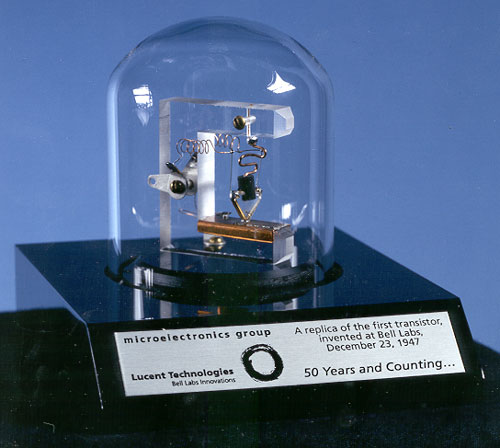
\includegraphics[width=0.45\linewidth]{images/book5/photo-first-transistor.jpg}

{\small نسخة طبق الأصل من أول ترانزستور (مختبرات بل، 1947، ملكية عامة): تماسّان ذهبيان مضغوطان على شظية من الجرمانيوم. أول آلة لنظرية العصابات --- وبالنسب، كل الآلات الأخرى.}
\end{omfigure}

\section{مسألة: استفتاء السطح}

\begin{problem}\label{pb:b3:electrons-in-solids:1}
\emph{استفتاء السطح.} جارك يقرر ما إذا كان
يسقّف بيته بألواح كهرضوئية، وقد عيّنك،
أنت الفيزيائي، حكمًا. واللوح المرشَّح: سيليكون،
\qty{2}{m^2}، بستين خلية على التسلسل، مقنَّن عند \qty{400}{W} تحت
\qty{1000}{W/m^2} المعيارية لضوء شمس الظهيرة.

\medskip\noindent\textbf{الجزء الأول --- ضوء الشمس يلقى الفجوة.}

\begin{enumerate}
  \item ضوء الشمس تقريبًا طيف حراري عند \qty{5800}{K}
        (\cref{ch:b3:photons-phonons}): احسب طاقة
        فوتوناته الذروية (بفين) بوحدة eV.
  \item وفجوة السيليكون \qty{1.12}{eV}: فما أطول
        طول موجي تستطيع خلية سيليكون حصاده؟
  \item ونحو خمس قدرة الشمس يصل في فوتونات
        دون الفجوة. فماذا يصيبها في اللوح؟
  \item ويُمتصّ فوتون أخضر عند \qty{2.5}{eV}: فكم من
        طاقته ينجو طاقةً لزوج إلكترون--ثقب، وأين
        تذهب البقية، وبأيّ سرعة؟
  \item واجمع البندين 3 و 4 في حكم الطيف: فنحو
        نصف القدرة الواردة يضيع قبل أن تبدأ أيّ إلكترونيات.
        اذكر قناتَي الفقد في جملة واحدة لكلٍّ.
  \item ولماذا يحتاج الفوتون إلى $\ge E_{\text{g}}$ أصلًا --- فما الذي
        يمنع امتصاص فوتونين بنصف الفجوة تعاقبًا
        سريعًا في السيليكون العادي؟
\end{enumerate}

\medskip\noindent\textbf{الجزء الثاني --- الوصلة محركًا.}

\begin{enumerate}[resume]
  \item كل خلية \omterm{prop:b3:electrons-in-solids:junction}{وصلة PN}. اشرح في ثلاث جمل
        كيف تحوّل منطقةُ الاستنزاف بمجالها الداخلي زوجًا مخلوقًا
        إلى تيار خارجي --- أيّ حامل يذهب في أيّ اتجاه، ولماذا لا يعيدان التحامهما ببساطة.
  \item ومع $N_{\text{a}} = N_{\text{d}} = \qty{1e22}{m^{-3}}$
        و $n_{\text{i}} = \qty{1e16}{m^{-3}}$، احسب
        $V_{\text{bi}}$ عند \qty{300}{K}.
  \item والخلية العاملة تعطي نحو \qty{0.6}{V}. فستون على
        التسلسل: ما جهد تشغيل اللوح؟
  \item ومن التقنين \qty{400}{W}، استنتج تيار
        التشغيل.
  \item وقدّر تدفق الفوتونات (فوتونات في الثانية) التي يمتصّها
        اللوح امتصاصًا مفيدًا، بأخذ $\sim\qty{2}{eV}$ لكل فوتون
        ممتَصّ، وقارنه بتدفق الإلكترونات الذي يقتضيه تيارك:
        فأيّ نسبة من الفوتونات الممتَصّة تعطي
        إلكترونًا مجموعًا؟
  \item والمردود المقنَّن: \qty{400}{W} من
        \qty{2000}{W} واردة. وفّق بين 20\,\% وبين ``نصف يضيع
        قبل الإلكترونيات'' في الجزء الأول: فأين تذهب النقاط
        الثلاثون الباقية؟
  \item ولماذا تعطي الخلية \qty{0.6}{V} لا كامل
        \qty{1.12}{V} للفجوة؟ (سمِّ الجاني في قانون
        الثنائي.)
\end{enumerate}

\medskip\noindent\textbf{الجزء الثالث --- السطوح الحقيقية.}

\begin{enumerate}[resume]
  \item ظهيرة شتوية صافية عند خط عرض $50^\circ$ تعطي
        ضوءًا عند ارتفاع $30^\circ$. احسب العامل الهندسي
        قياسًا إلى الورود الناظمي على لوح
        أفقي.
  \item وورقة بيانات اللوح تذكر $-0.4\,\%/\text{K}$ من الخرج:
        ولوح سطح أسود يبلغ \qty{65}{\celsius} في الصيف.
        فكم من التقنين ينجو؟
  \item واشرح فقد درجة الحرارة على ضوء
        \cref{exo:b3:electrons-in-solids:12}(د).
  \item ومدخنة تظلّل خلية واحدة من الستين. فلماذا يستطيع ذلك
        خنق سلسلة التسلسل كلها --- وماذا تفعل طبيعة
        الخلية الثنائية بالخلية المظلَّلة المسكينة؟
  \item ويصل الصنّاع \emph{ثنائي تجاوز} عبر كل
        سلسلة جزئية: اشرح وظيفته في جملة واحدة.
  \item ومتوسَّطًا على الأيام والطقس، يعطي السطح
        \qty{15}{\percent} من القدرة المقنَّنة. قدّر الطاقة السنوية
        من لوح \qty{400}{W} بالكيلوواط-ساعة.
\end{enumerate}

\medskip\noindent\textbf{الجزء الرابع --- الحكم.}

\begin{enumerate}[resume]
  \item بسعر \qty{0.25}{euros} لكل \unit{kWh}، فكم يكسب اللوح
        في السنة؟ ومع كلفة تركيب مقدارها \qty{300}{euros}،
        فما زمن الاسترداد؟
  \item واستغرق صنع اللوح نحو \qty{500}{kWh}
        (فالسيليكون يُنقّى بالصهر): فمتى يكون قد سدّد طاقته هو؟
  \item ويسأل جارك لماذا لا يمكن جعل اللوح
        ``أسود فحسب'' ليلتقط الخُمس دون الفجوة. أجب
        بنظرية العصابات في جملتين.
  \item ثم يسأل لماذا لا يُكدَّس لوح ثانٍ أضيق فجوةً
        تحته: أجب على ضوء
        \cref{exo:b3:electrons-in-solids:12}(ج) --- وسمِّ
        العائق العملي.
  \item وبعد ثلاثين سنة يكون اللوح قد خبا إلى 85\,\% من
        تقنينه. فأيّ أشرار مجهريين من هذا الفصل
        (تذكّر ما يحدّ $\tau$، وما تخشاه الوصلات)
        يُشيخون خليةً على نحو معقول؟
  \item وقدّم خلاصة الحكم في أربعة أسطر: فيزياء الفجوة
        تضع الحصاد، والوصلة تحوّله، وتوصيل
        التسلسل ودرجة الحرارة يفرضان عليه ضريبة، والدفتر --- الطاقة
        واليوروات --- يُغلق لصالح اللوح.
\end{enumerate}
\end{problem}
